\section{Программные средства моделирования \\
  и автоматизированного проектирования \\
  конструкций РЭС}

% KiCAD

Из-за моей приверженности к
свободному программному обеспечению ~\cite{GNU-philosophy},
мною была выбрана САПР
с открытым исходным кодом \textit{KiCAD} ~\cite{kicad-license}.


Для меня такой выбор связан,
с используемой мной в настоящей момент операционной системой,
а также тем, этическим соображениям, которые,
будучи кратко сформулированы,
звучат как: Если пользователи не контролируют программу,
программа контролирует пользователей ~\cite{ufair-nonfree-programs}.

% PCB doc screenshot

\begin{figure}[H]
  \centering
  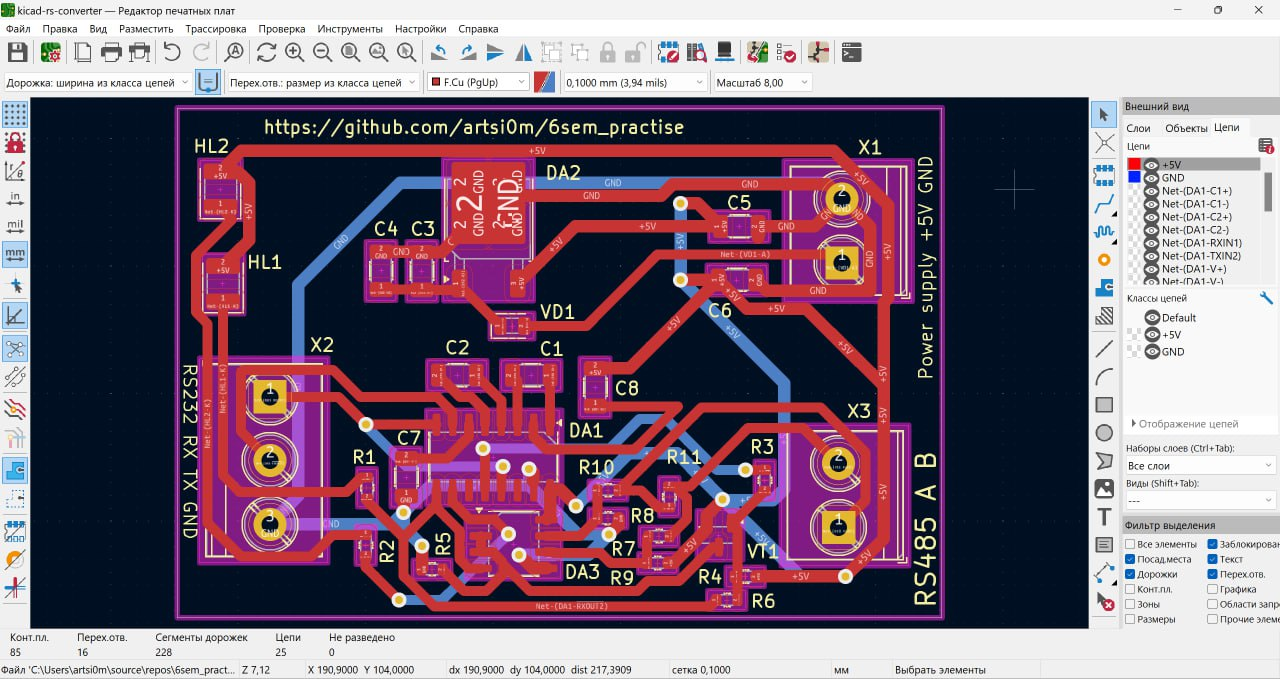
\includegraphics[scale=0.4]{kicad-pcb-doc-with-rs-converter.jpg}
  \caption{Снимок экрана с ПП открытой в kicad-pcbdoc}
\end{figure}


Данная САПР, на настоящий момент,
является одним из самых передовых решений,
среди всех свободных САПР.
Примечательно также, что его разработку также спонсировал \textit{CERN}
(Европейский Институт Ядерных Исследований) ~\cite{kicad-sponsors}.

Другой причиной выбора мною данной САПР при разработке,
был используемый текстовой формат файлов,
при котором данные в документах САПР представлены
не иначе как Эс-Выражения (англ. \textit{S-Expressions})
~\cite{kicad-sexpr}. В отличие от бинарных файлов документов,
используемых в \textit{Altium Designer},
файлы созданные при разработке печатной платы,
в \textit{Kicad} за счёт их текстовой природы
можно размещать в репозитории системы контроля версий git.
Git это распределённая система контроля версий \cite{git-dvcs}
исходного кода программ. Из-за своего формата,
файлы \textit{KiCAD} могут быть обработаны,
как исходный код программы. Это, с свою очередь,
позволяет работать с нескольким людям,
с различными версиями одного проекта
и при этом добиваться\\
синхронизации его между всеми участниками,
в определённый момент времени.

\begin{figure}[H]
  \centering
  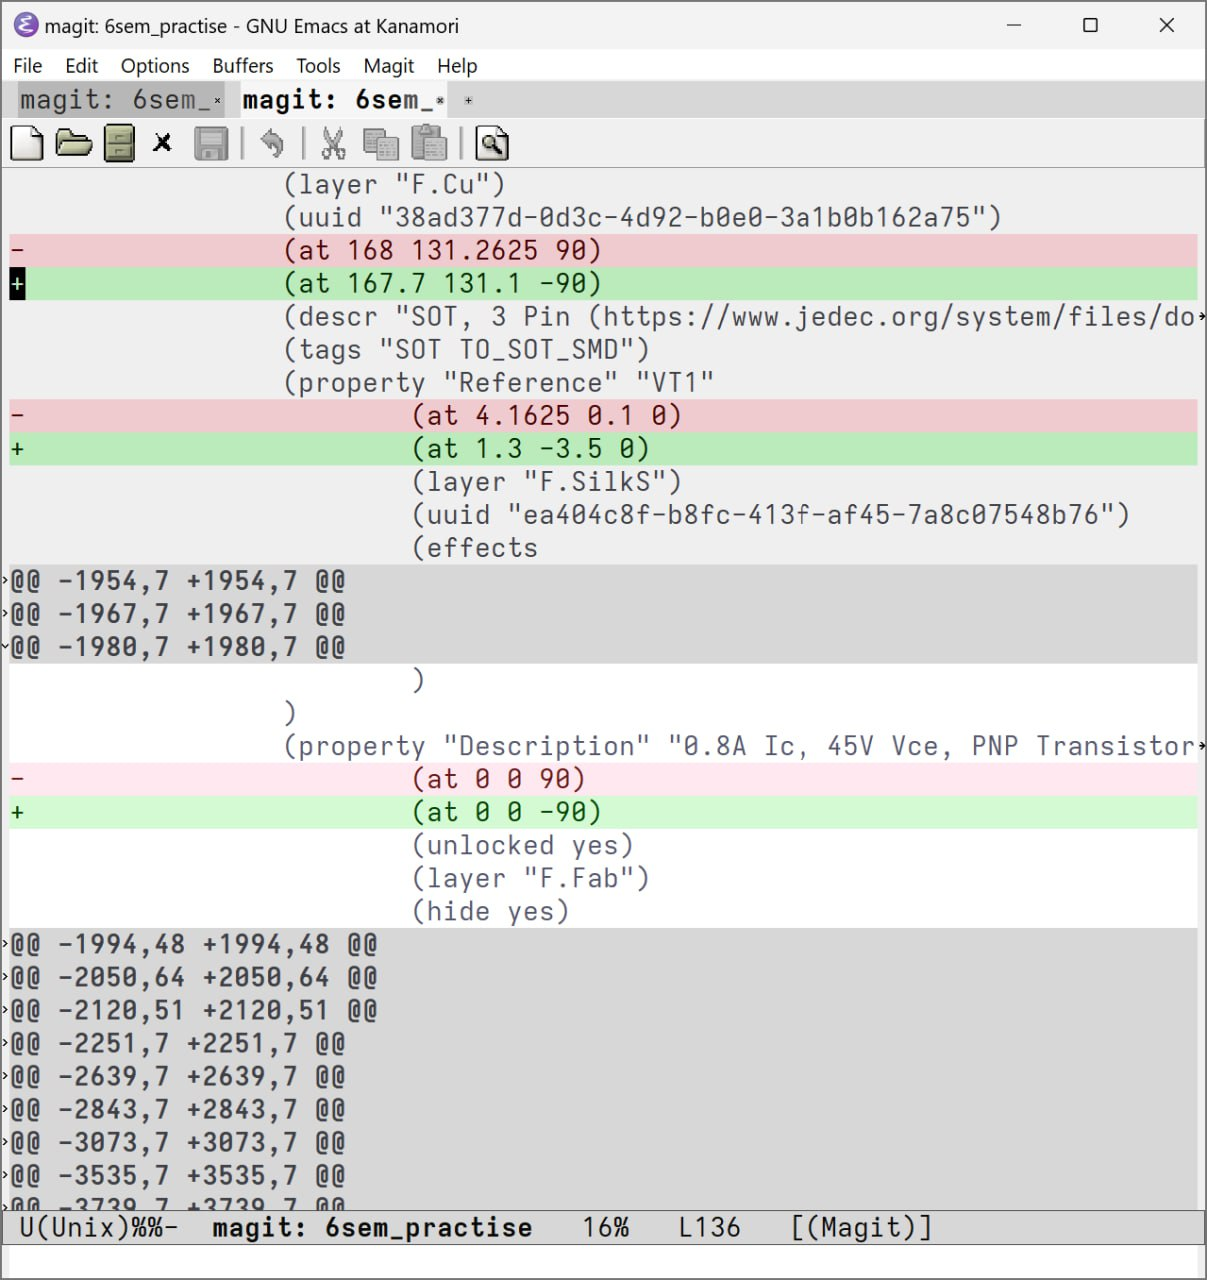
\includegraphics[scale=0.5]{magit-6-sem-practise.jpg}
  \caption{Снимок экрана с окном magit,
    установленный в расширяемый редактор текста GNU/Emacs
    клиент системы контроля версий git.
    Видно, как magit может распознать изменения файла трассировки печатной платы,
    как добавление и удаление строк.}
\end{figure}


Например в одном репозитории печатной платы,
схемотехник может в файле принципиальной схемы
создать принципиальную схему устройства,
а конструктор в свою очередь, синхронизировав файл
через \textit{git} может,
основываясь на схеме составленной схемотехником,
трассировать печатную плату. Более того, используя
так называемый монорепозиторий, как подход работы с \textit{git},
в одном репозитории можно содержать как печатную плату,
так и исходный код прошивки микроконтроллера,
используемый в ней.

В данной САПР было осуществлено создание
актуальной принципиальной cхемы устройства,
а также трассировка печатной платы, на основе связей между элементами,
импортированных из схемотехнической
части программы \textit{kicad-eeschema} ~\cite{kicad-doc-eeschema}.
% kicad-doc-eeschema
% link to some of the oficial v8.0 docs on site

% Скриншот eeschema
% Cкриншот pcbdoc
% SimulIDE, KTechLab Proteus

Во время разработки принципиальной схемы печатной платы,
была допущена ошибка, из-за которой транзистор,
размещённый на принципиальной схеме был подключен не теми выводами,
которые были обозначены на изначальной модернизируется
принципиальный схеме.
О своей оплошности я был осведомлён уже в тот момент,
когда выслал файлы по почте в отдел производство.
Я был проинформирован о недочёте в схеме начальником производственного отдела.
Это дало мне ценный урок:
при любых сомнениях в схемотехнической части разрабатываемого устройства,
следует использовать САПР,
с возможностью симуляции сложных логических схем или микроконтроллеров.
Среди изученных мною ранее
таковой является \textit{Proteus} ~\cite{Proteus-Simulation}.
% Proteus-About
% Proteus site

Её аналог в мире свободного программного обеспечения - \textit{SimulIDE} ~\cite{SimulIDE}.
%

Для разработки данной печатной платы было достаточно
использование САПР ПП \textit{KiCAD},
однако стоит отметить, что использование специальных САПР симуляторов,
например \textit{Proteus} или \textit{KiCAD} существенно бы ускорило,
процесс изготовления и введения устройства в эксплуатацию
за счёт экономии времени на этапе исправления ошибок в принципиальной схеме.

\newpage

% Local Variables:
% compile-command: "sh build.sh"
% End:
